\section{Introdução}

\begin{frame}{Introdução - contexto}
\textbf{Objetivo:}
\begin{itemize}
    \item Organizar bobinas em um galpão de forma a \textbf{minimizar os movimentos futuros} e, consequentemente, o \textbf{gasto energético}.
    \item Buscar uma \textbf{distribuição ótima} para atender às demandas previstas.
\end{itemize}

\vspace{0.4cm}
\textbf{Contexto Operacional:}
\begin{itemize}
    \item Galpão industrial com dois níveis de armazenamento.
    \item Movimentação realizada por uma ponte rolante (carregada ou vazia).
    \item Cada movimentação consome tempo e energia, dependendo da origem e destino.
\end{itemize}

\vspace{0.4cm}
\textbf{Dinâmica do Sistema:}
\begin{itemize}
    \item Bobinas possuem janelas de \textbf{entrada} e \textbf{saída} definidas.
    \item Movimentações internas são possíveis para reorganização.
    \item O modelo decide \textbf{quando mover, o que mover e para onde mover}.
\end{itemize}
\end{frame}

%%%%%%%%%%%%%%%%%%%%%%%%%%%%%%%%%%%%%%%%%%%%%%%%%%%%%%%%%%%%%%%%%%%%%%%%%%%%%%%%%%%%%%%%%

\begin{frame}{Introdução - armazenamento}
    \begin{figure}
        \begin{figure}
            \centering
            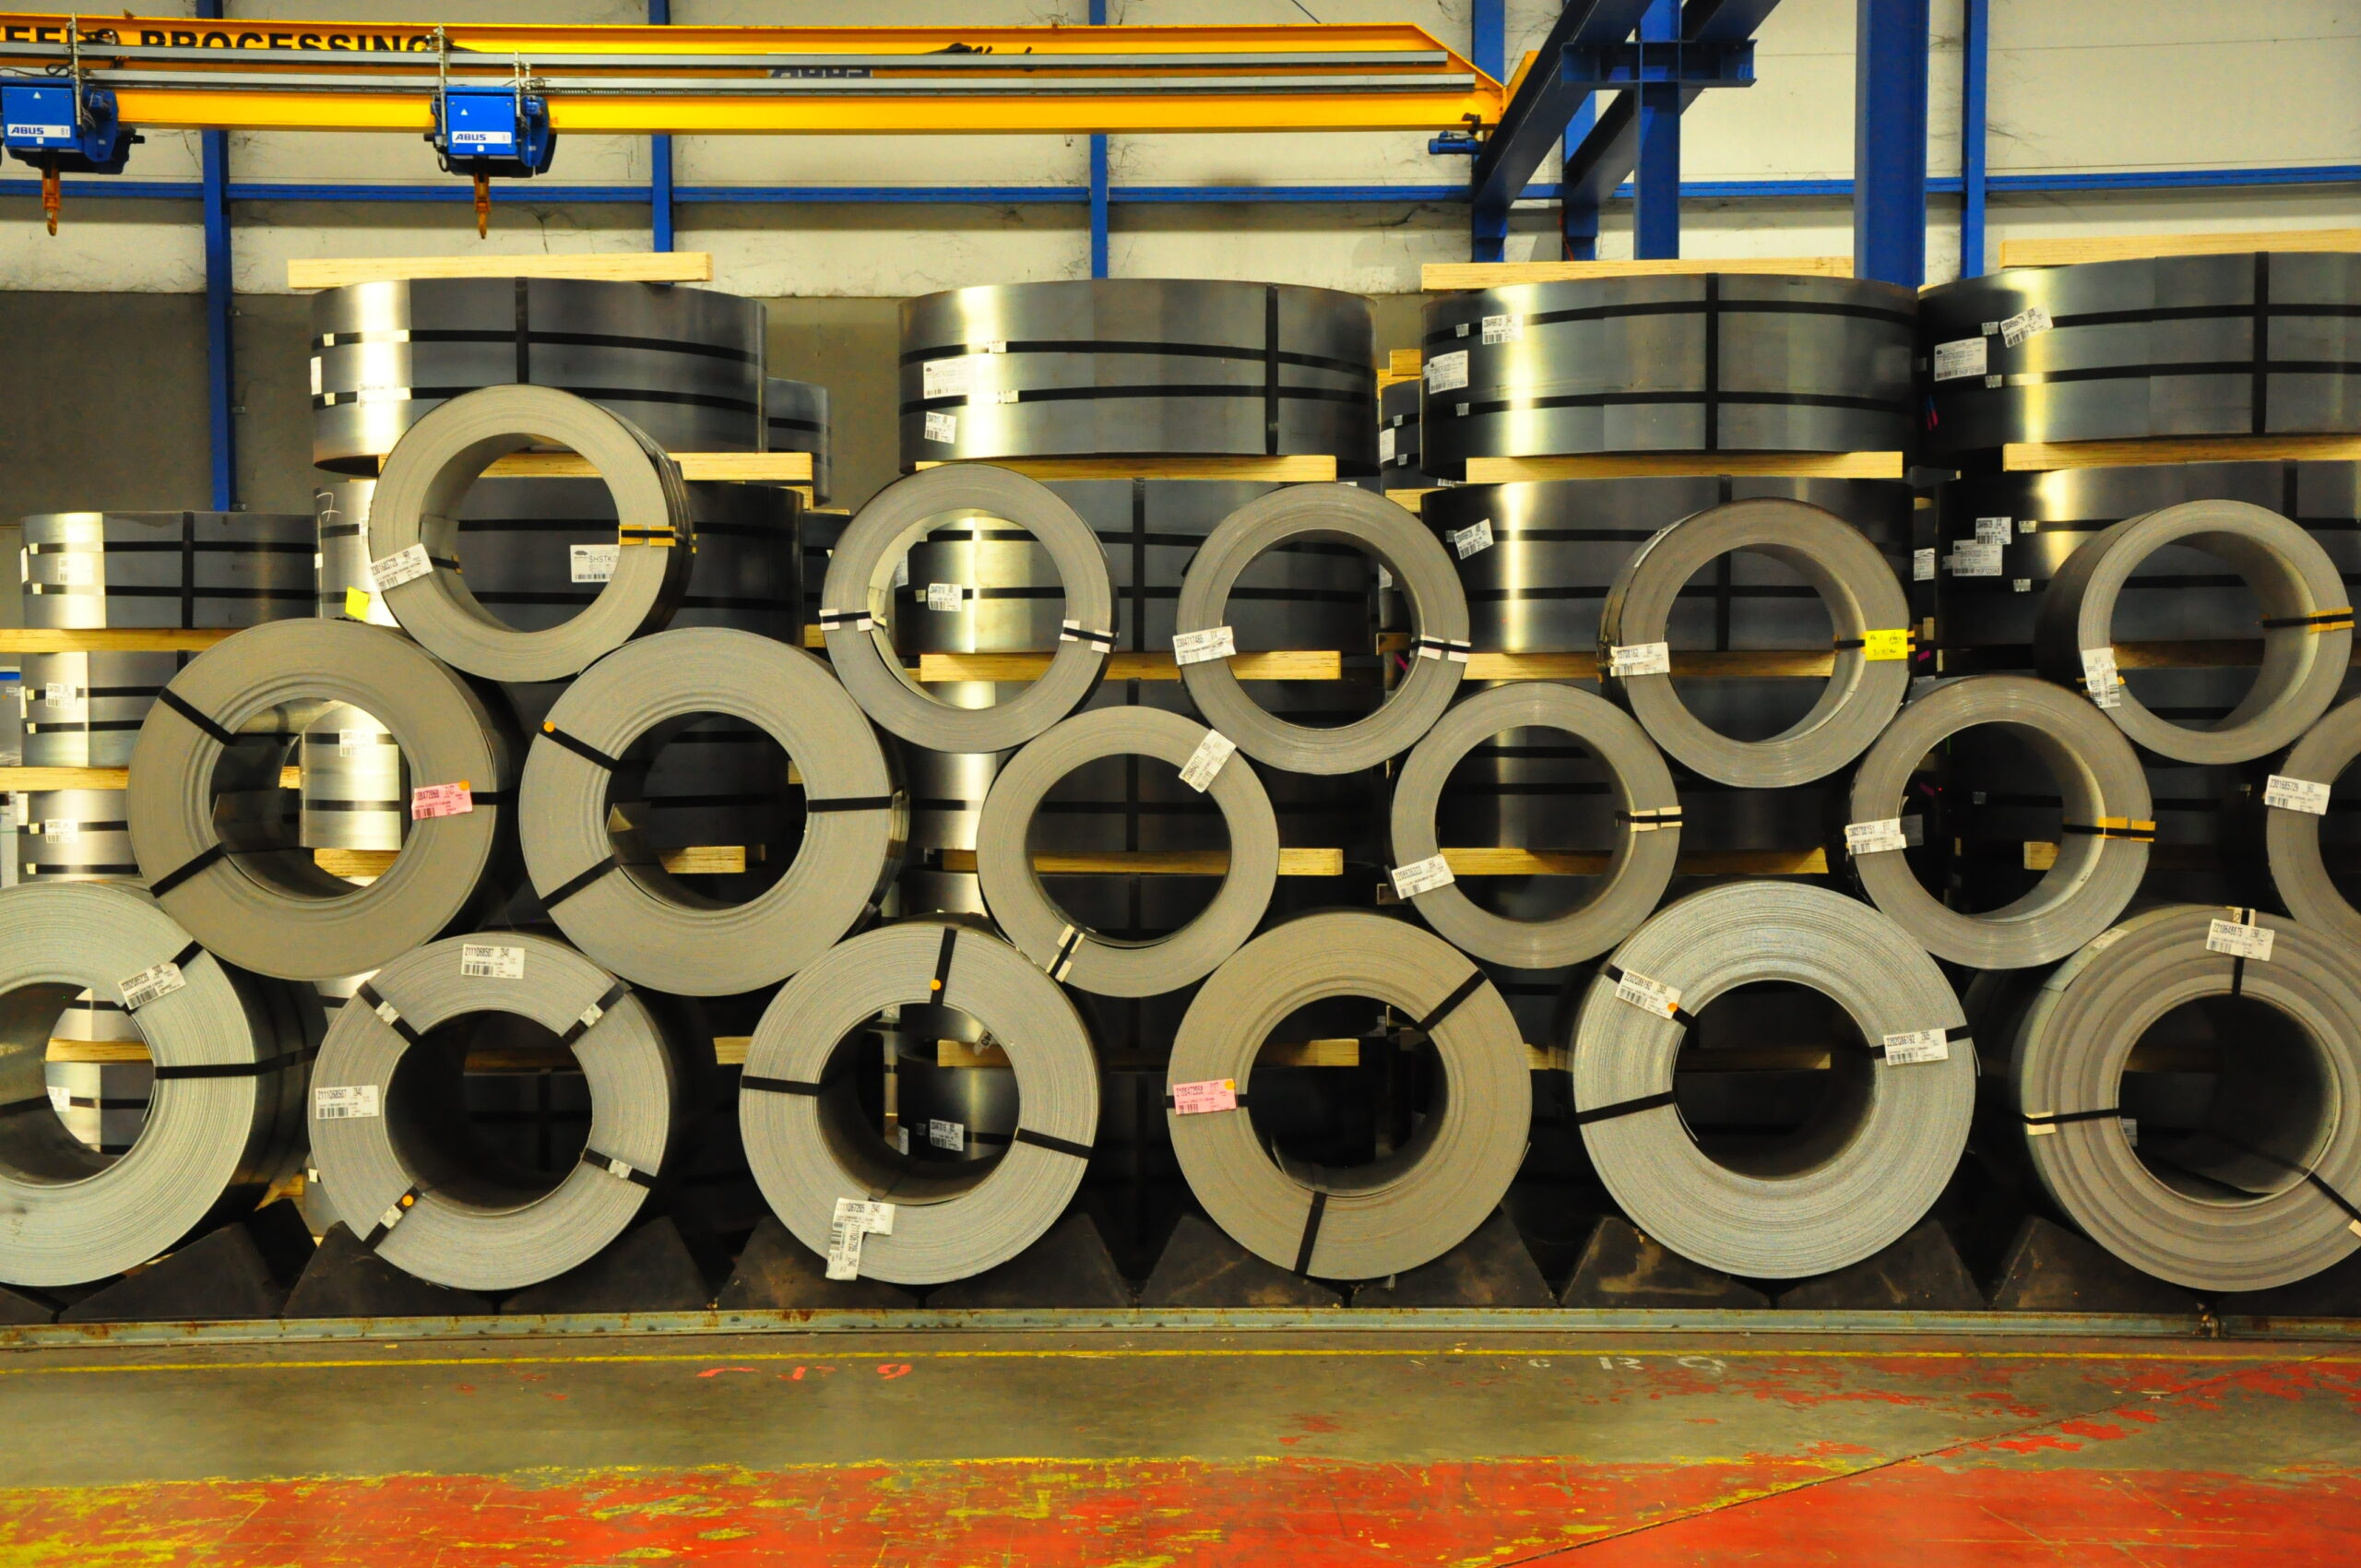
\includegraphics[width=0.5\linewidth]{imagens/rolled-coils-in-storage.png}
            \caption{Bobinas diferentes em armazenamento}
            \label{fig:bobinas-armazenamento}
        \end{figure}
    \end{figure}
\end{frame}